\section{PHASE-TTC: independent estimates, shared phase}
\label{sec:train40}

\subsection{Deployed model composition}

PHASE-TTC deploys a causal chain of nine fitted components comprising four modality-specific producers, two pairwise temporal heads, two context refiners, and one fusion head. RGB and events each use a transport-trained baseline producer (A5) and a coarse-to-fine producer (C2F). The pairwise readouts extract phase features from their A5 representations, after which the context refiners incorporate temporal history. The fusion head anchors its correction on the refined RGB estimate. Figure~\ref{fig:deployed-architecture} traces this path; the five auxiliary rotations serve training only. \evidence{M22,M23}

\begin{figure}[htbp]
  \centering
  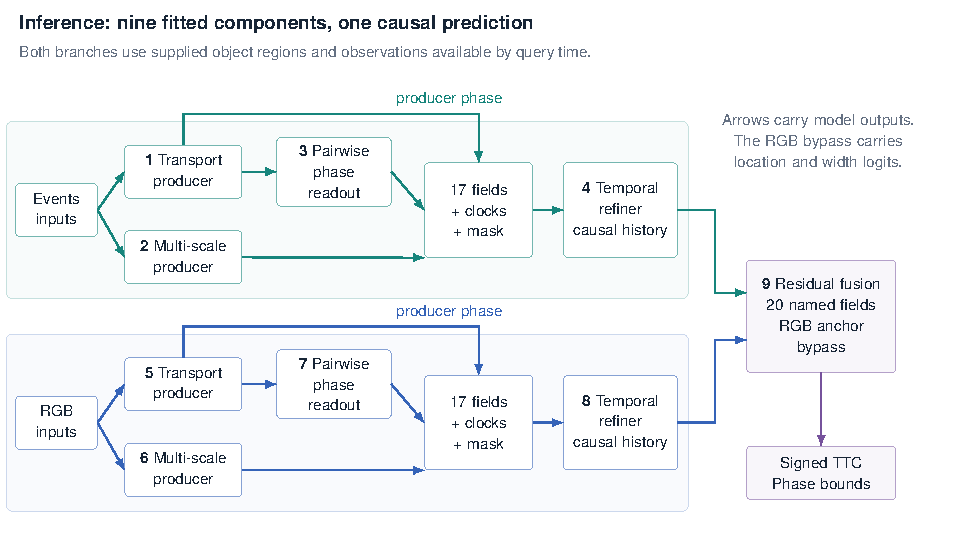
\includegraphics[width=\linewidth]{figures/publication_architecture.pdf}
  \caption{\textbf{Causal nine-component inference graph.} Supplied object regions feed parallel RGB and event producers, pairwise temporal heads, and temporal refiners. Twenty named fields enter the final RGB-anchored fusion head. \evidence{M03,M22,M23}}
  \label{fig:deployed-architecture}
\end{figure}

\begin{table}[htbp]
\centering\scriptsize
\caption{The nine fitted components in the submitted inference chain. RGB and event branches share the listed functional roles but have separate fitted weights. All targets and privileged supervision belong to fitting; inference uses sensor observations and supplied object regions.}
\label{tab:component-contracts}
\begin{tabularx}{\linewidth}{@{}p{.15\linewidth}p{.23\linewidth}p{.26\linewidth}X@{}}
\toprule
Components & Inputs & Architecture and outputs & Fitting signal \\
\midrule
Two transport producers & Shared-region temporal crops; observed endpoint intervals & Convolutional endpoint encoder, local feature correlation and scale residual; dense features, geometry and TTC & TTC, foreground/box geometry and RGB-derived relational distillation \\
Two coarse-to-fine producers & Same modality-specific crop contract & Two-scale local transport with a learned gate; alternate motion estimate & Producer objective with geometric and relational supervision \\
Two pairwise readouts & 133 fields derived from each transport producer's endpoints & LayerNorm, width-128 GELU MLP and scalar phase output & Smooth-L1 phase regression \\
Two context refiners & 17 fields per observation, four timing fields and validity mask & Two-layer width-160 GRU; phase correction around current expert median and phase widths & Group-weighted phase error, quantile losses and expert-relative costs \\
One fusion head & Ten named fields per modality; RGB anchor and width logits & Two width-32 layers with LayerNorm/SiLU; location and width corrections & Group-weighted phase error and quantile losses on out-of-fold features \\
\bottomrule
\end{tabularx}
\end{table}


\subsection{Object coordinates and causal history}

Each query includes supplied object coordinates. A common spatial frame covers both endpoint regions and preserves apparent scale change, which independent tight crops can erase. The evaluated system therefore assumes external localization.

Both branches use observations available by query time \(t\), with up to 650\,ms of causal history. Runtime begins at its declared measurement boundary and ends when the host receives the complete TTC output. Figure~\ref{fig:causal-history} separates the sensing interval from response time; its observation marks are schematic. \evidence{M03,M22,L43,L44}

\begin{figure}[H]
  \centering
  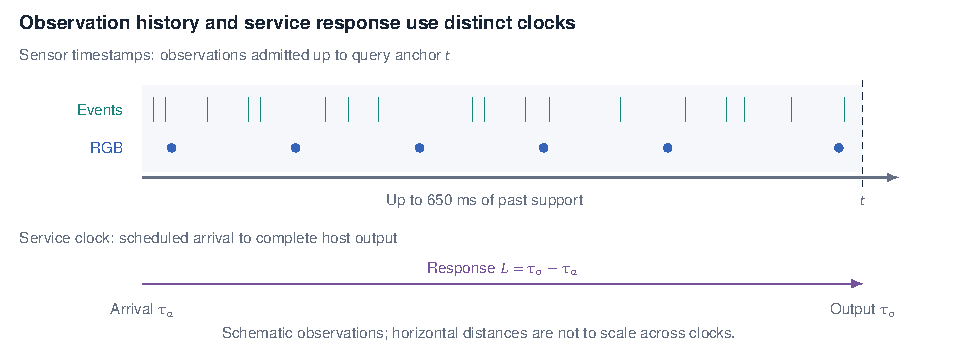
\includegraphics[width=\linewidth]{figures/publication_history.pdf}
  \caption{\textbf{Causal support and response-time boundaries.} RGB and event observations precede the sensor-time query anchor \(t\). A separate service clock measures from scheduled arrival \(\tau_a\) to complete host output \(\tau_o\); the two axes are schematic.}
  \label{fig:causal-history}
\end{figure}

\subsection{Phase as a shared motion coordinate}
Let $T$ denote signed TTC, positive for approach and negative for recession. With reference interval $d_0=0.1\,\mathrm{s}$, we use
\begin{equation}
 \phi(T)=-\log(1-d_0/T),\qquad T<0\ \text{or}\ T>d_0.
 \label{eq:phase-main}
\end{equation}
For large $|T|$, $\phi(T)\simeq d_0/T$: slow approach and recession lie near zero. Sensitivity increases toward the positive domain boundary $T=d_0$. This is a shared signed coordinate, not a removal of the near-contact singularity. The benchmark evaluates error in this coordinate; Section~\ref{sec:protocol} defines its weighting.

\subsection{A residual correction around RGB}
Each modality $m\in\{R,E\}$ exposes a vector $\mathbf{x}_m\in\mathbb{R}^{10}$: a raw phase location, the emitted point phase, three expert phases, four timing fields, and a valid-history count normalized by eight. The hidden state stays within its own branch. Let $D=\operatorname{diag}(\alpha^{-1}I_5,I_5)$, with $\alpha=0.03$. The fusion input is
\begin{equation}
 \mathbf{z}=[D\mathbf{x}_R;D\mathbf{x}_E]\in\mathbb{R}^{20}.
\end{equation}
Thus corresponding coordinates have the same meaning across modalities, while timing and support keep their native scaling. Appendix~\ref{sec:physical-fusion-fields} defines the timing fields precisely.

The residual network $g_\theta:\mathbb{R}^{20}\to\mathbb{R}^{3}$ uses two width-32 layers with LayerNorm and SiLU activations:
\begin{equation}
 \mathbf c=g_\theta(\mathbf z).
\end{equation}
Its 1,955 parameters include the affine maps and both LayerNorms. Given the RGB raw-location anchor $\ell_R$ and width logits $\mathbf w_R$, the corrected location and widths are
\begin{align}
 \ell_F&=\ell_R+\alpha c_0,\\
 [\sigma_l,\sigma_u]^\top&=\alpha\operatorname{softplus}(\mathbf w_R+[c_1,c_2]^\top).
\end{align}
Zero initialization of $W_3$ and $\mathbf b_3$ starts optimization at the RGB anchor. The factor $\alpha$ scales the residual; it imposes no bound on $c_0$. The widths parameterize phase-interval endpoints and require empirical calibration before a probabilistic interpretation.

For a finite emitted prediction, we first clamp $\ell_F$ to $[\phi_{\min},\phi_{\max}]$, where $\phi_{\min}=-\log 2+10^{-6}$ and $\phi_{\max}=8$, then compute
\begin{equation}
 q_F=\frac{1-\exp(-\operatorname{clip}(\ell_F,\phi_{\min},\phi_{\max}))}{d_0},
 \qquad \widehat T=\frac{\operatorname{sgn}_{+}(q_F)}{\max(|q_F|,1/60\,\mathrm{s}^{-1})}.
\end{equation}
Here $\operatorname{sgn}_{+}(0)=1$, so zero phase emits $+60\,\mathrm{s}$. The rate floor limits the magnitude of emitted TTC near zero expansion. Figure~\ref{fig:fusion-interface} shows the anchor and correction paths; Appendix~\ref{app:implementation} gives the exact array layout, stable numerical inverse, and interval bounds. \evidence{M22,R02}

\begin{figure}[htbp]
\centering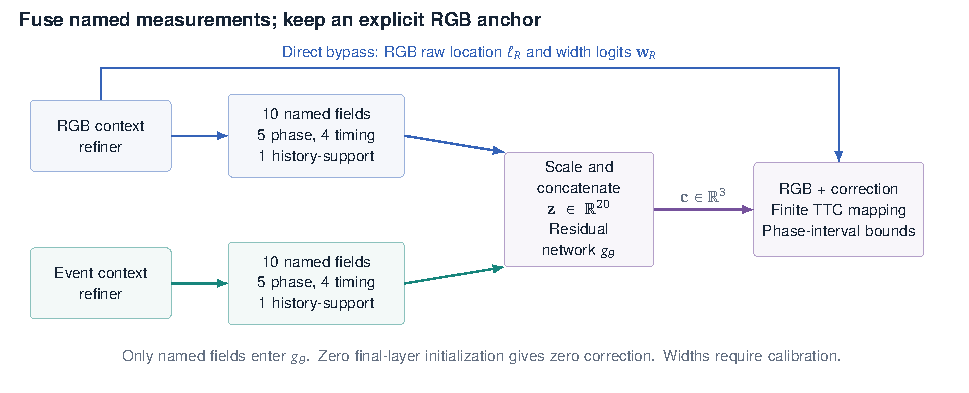
\includegraphics[width=\linewidth]{figures/publication_fusion.pdf}
\caption{\textbf{Shared measurements and an RGB anchor.} The two ten-field descriptors feed the residual network. RGB location and width logits also reach the output directly; only the learned correction passes through the network. Hidden features do not enter the fusion input.}
\label{fig:fusion-interface}
\end{figure}

\subsection{Submission coverage and benchmark status}

The official submission contains finite predictions without fallback for 6,762 query tokens across twelve sequences: 5,805 physical queries and 957 aliases. Aliases identify repeated physical queries and do not represent additional inference work.

Section~\ref{sec:official} reports the test result for this graph. Section~\ref{sec:design-analysis} holds the final upstream features fixed and refits matched correction heads to test their use of event information. \evidence{L44,B01,B02}